%%%%%%%%%%%%%%%%%%%%%%%%%%%%%%%%%%%%
\chapter{Literature Review} 
\label{chap:Literature_Review}
%%%%%%%%%%%%%%%%%%%%%%%%%%%%%%%%%%%%

\comment{

Use your literature review to help the reader to understand the value and the interest in your project.  You should look for related works already published that either support the merit of your project, or provide the background understanding/information to make your new claims.  Try to avoid writing a "catalogue" of related works (e.g this would have little of your own insight added).  Instead, describe to the reader why the related work is interesting or relevant to your own work.  What did they achieve?  What did they overlook?  It is highly recommend you finish your Literature Review with a final subsection "Summary", where you may wish to formulate highly specified research questions or hypotheses, or assert the need for your Research Methodology (next chapter).  

introduction
literature review
implementation
research methodology
results




\section{This is a section}
\subsection{This is a subsection}
\subsubsection{This is subsubsection}

%%%%%%%%%%%%%%%%%%%%%%%%%%%%%%%%%%%%
% Figure with subfigures
%%%%%%%%%%%%%%%%%%%%%%%%%%%%%%%%%%%%

\begin{figure}[htb]
\centering
\begin{subfigure}[t]{.5\textwidth}
  \centering
  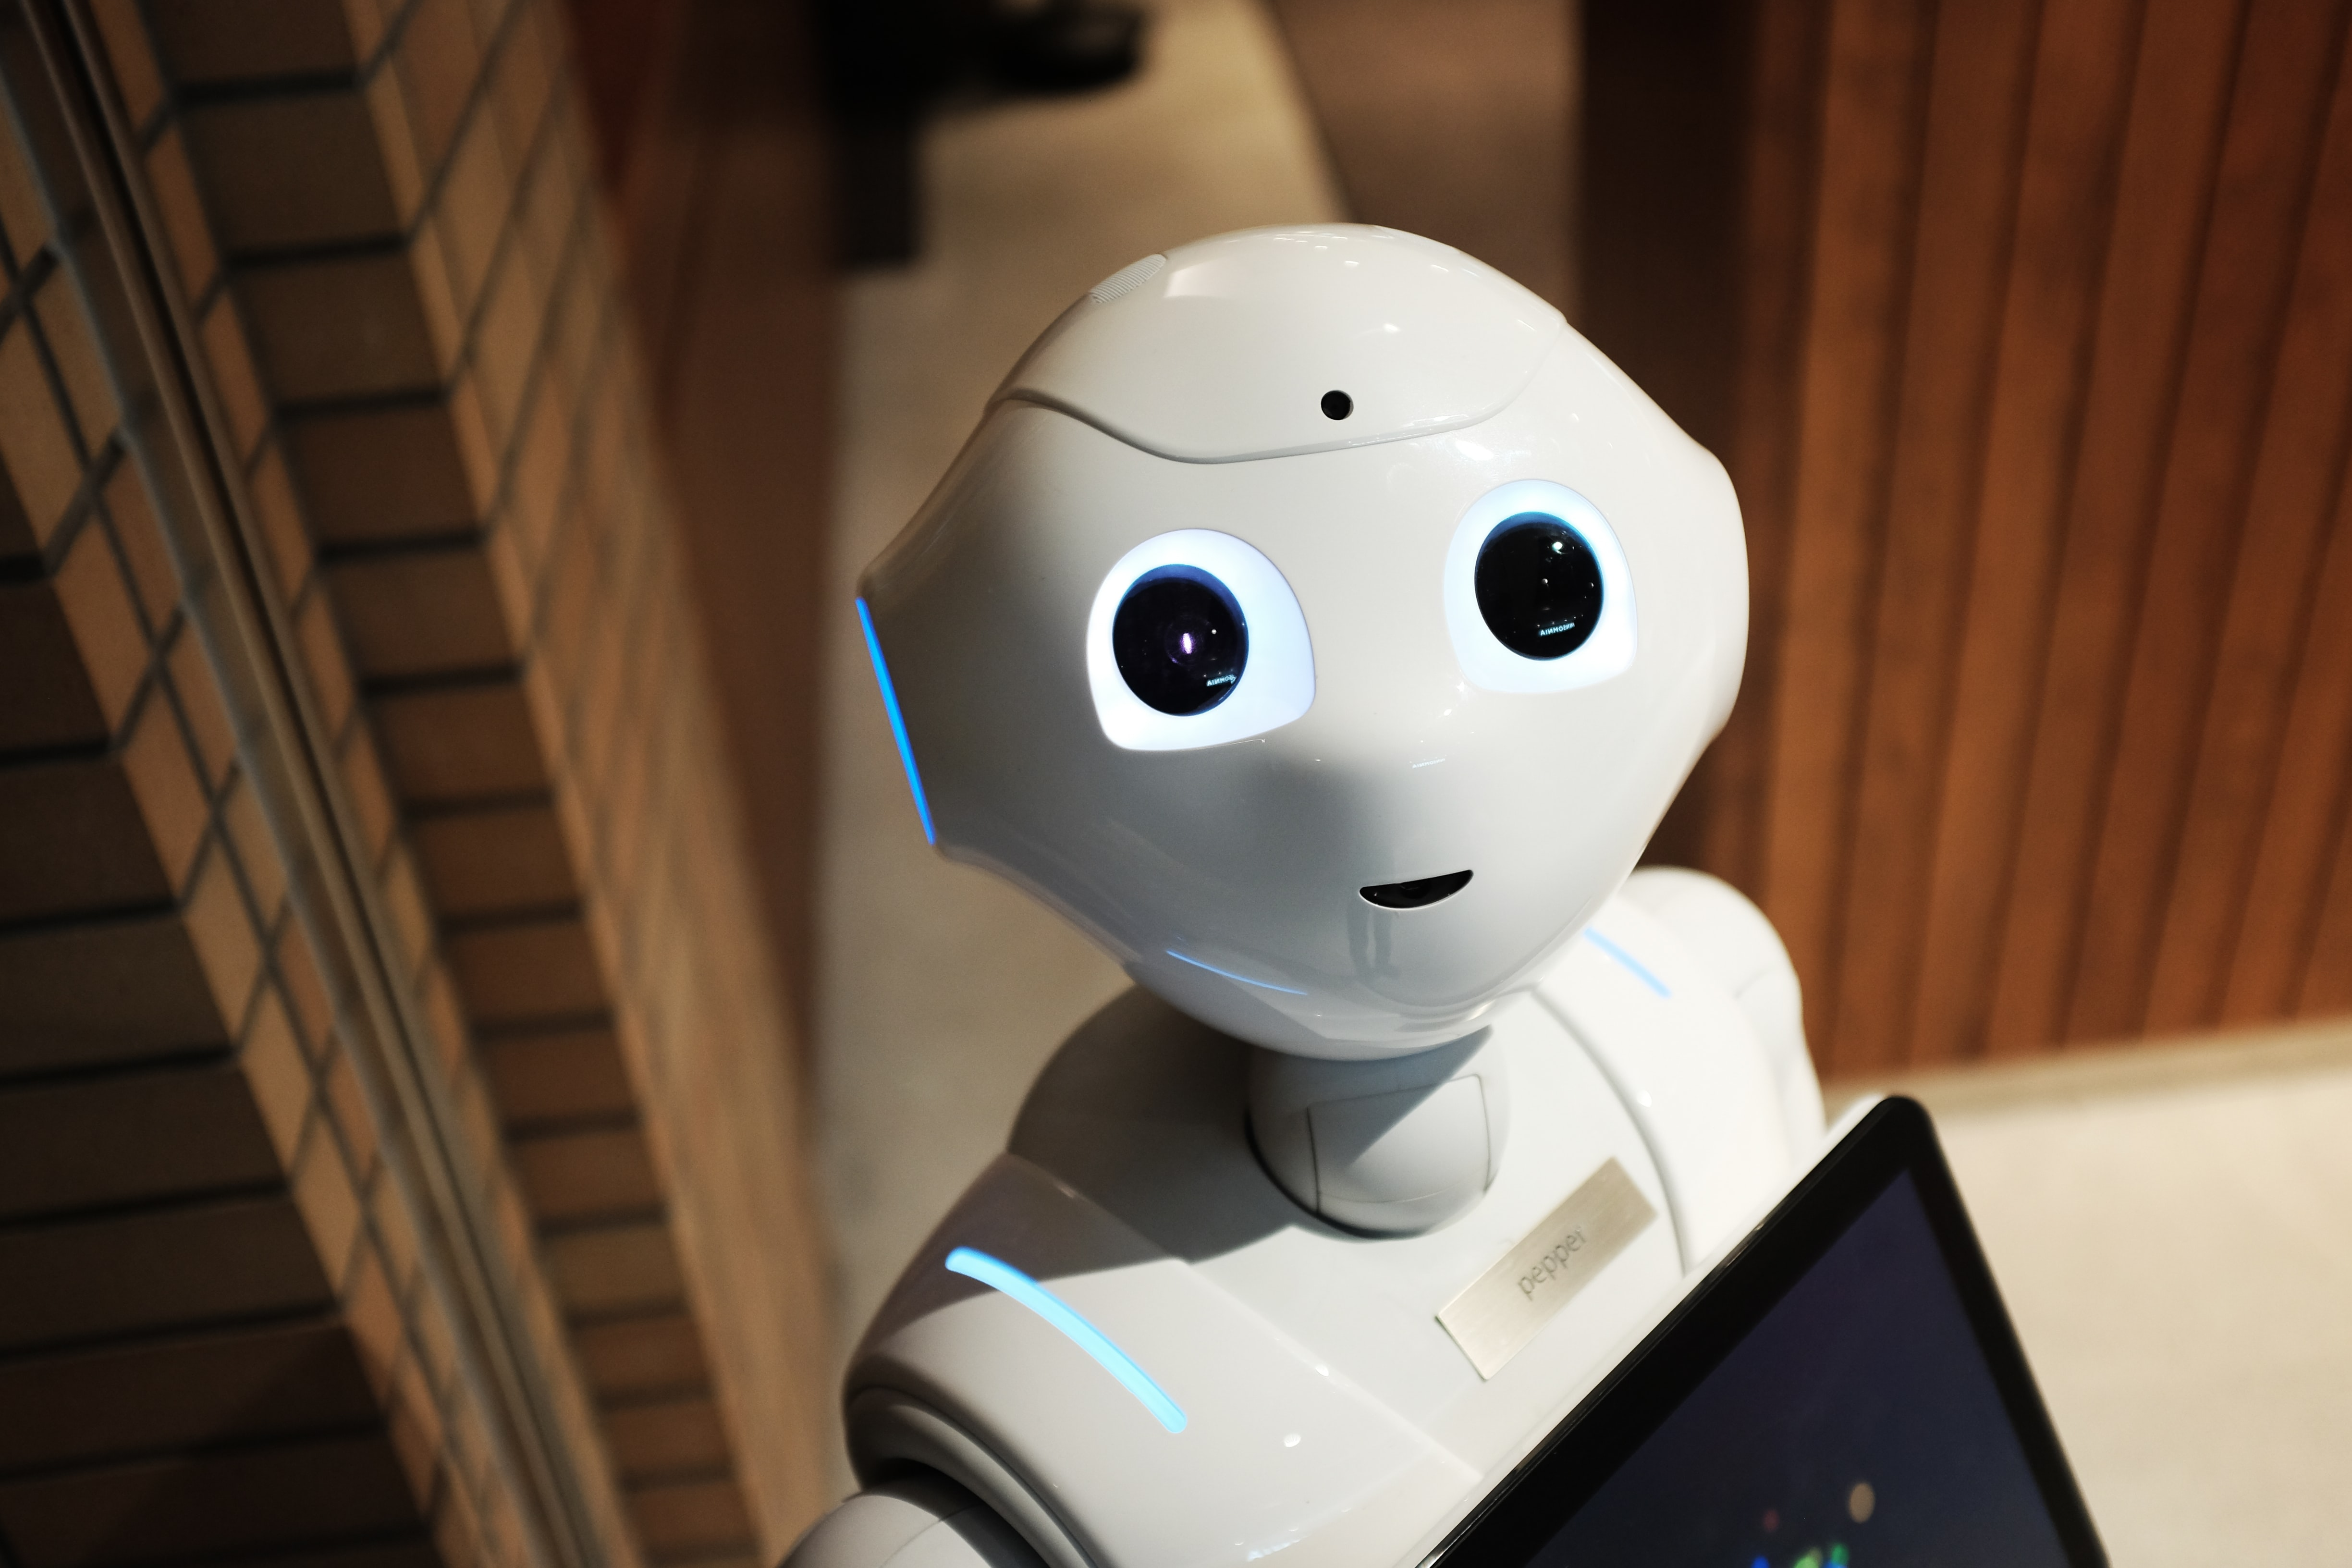
\includegraphics[height=4.5cm]{figures/Robot_1.jpg}
  \caption{\label{fig:left_robot} This is a robot.}
  \label{fig:theoretical}
\end{subfigure}%
\begin{subfigure}[t]{.5\textwidth}
  \centering
  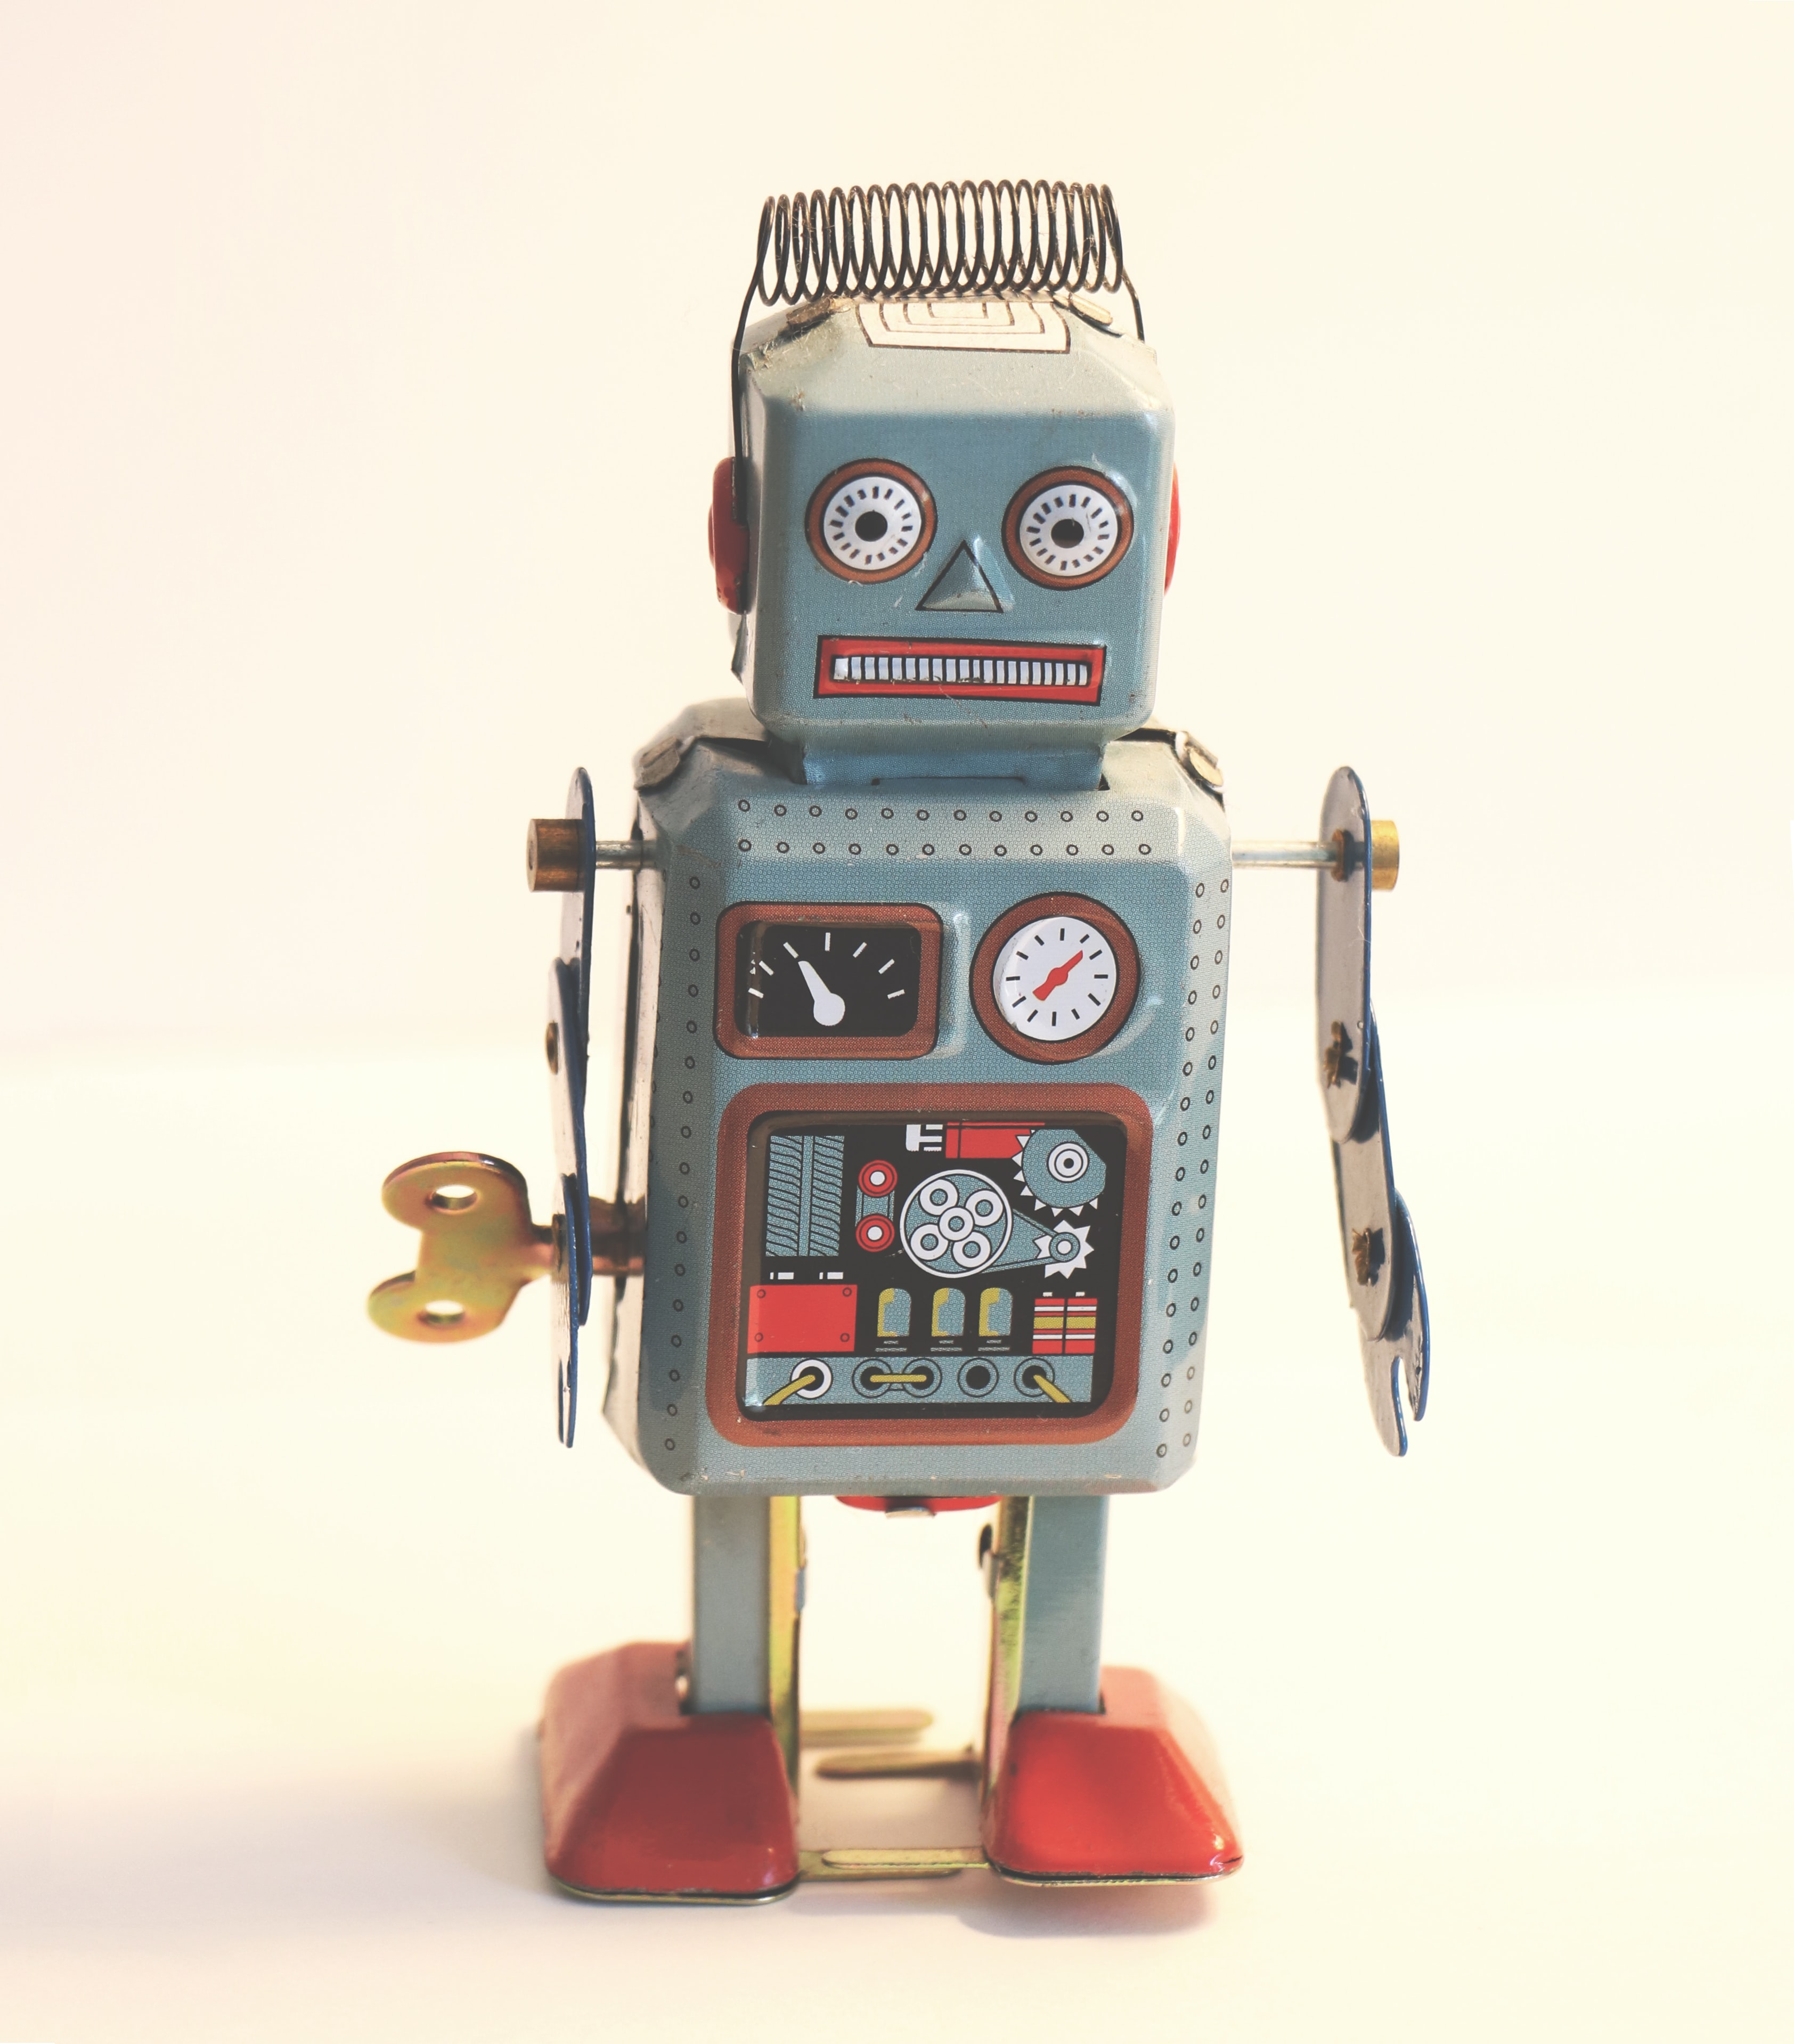
\includegraphics[height=4.5cm]{figures/Robot_2.jpg}
  \caption{\label{fig:right_robot} This another robot.}
  \label{fig:practical}
\end{subfigure}
\caption{\label{fig:two_robots} These are two robots}
\label{fig:test}
\end{figure}

For example, \cite{Robots2020} discusses the two robots depicted in Figure \ref{fig:two_robots}. There is a robot in Figure \ref{fig:left_robot} and another robot in Figure \ref{fig:right_robot}.

}

% 记得插一句关于本节要讲什么的总结

\section{STDMA Explained}

As previously mentioned in Section \ref{sec:Why STDMA?}, STDMA \cite{STDMA} allows multiple agents to 
share the same channel for communication without centralised control. The main assumption of this protocol
is that all devices have synchronised clocks. In practice, this is achieved through GPS \cite{STDMA_2}.

\textbf{The core idea of STDMA can be summarized as follows:} Represent continuous time with repeating
frames, each consisting of an euqal number of discrete slots. Agents constantly monitor channel information,
attempting to occupy a free slot in the frame for themselves. Once an agent secures a slot, it can broadcast
its information in that slot of every frame.

Agents using STDMA have \textbf{four phases}, which are arranged in chronological order as follows:

% 加个frame和slot的示意图?

\begin{enumerate}
  \item \textbf{Initialisation}: Agents in this phase have not yet joined the network. The agent listens to an entire frame and determines the current slot allocation.
  \item \textbf{Network Entry}:  Randomly choose an unallocated slot to broadcast their existence and reserve one slot for the next phase.
  \item \textbf{First Frame}: Use the slot reserved in the previous phase to reserve more slots for themselves. The number of reserved slots depends on the size of the data packet that the device needs to send.
  \item \textbf{Continuous Operation}: Use the previously reserved slot to work normally. If some slots are released or more slots are needed, reapply for slots.
\end{enumerate}

Although the above description omits some details (such as slot choosing methods,
 calculation of required number of slots, etc.), it is clear that
\textbf{the core of STDMA is the strategy of finding and reserving unallocated slots}.

This protocol also has some limitations, such as:
\textbf{(1)} Collision: In Network Entry phase, multiple devices may accidentally choose the same unallocated slot to broadcast their existence.
 \textbf{(2)} Capacity: When the slots are not enough, conflicts will inevitably occur. There are some studies \cite{STDMA_improv1,STDMA_improv2} that proposed improvements to the above limitations, but this is not the focus of this project.

\section{MAPF Algorithm Review}